%%%%%%%%%%%%%%%%%%%%%%%%%%%%%%%%%%%%%%%%%%%%%%%%%%%%%%%%%%%%%%%%%%%%%%
% Slides
%%%%%%%%%%%%%%%%%%%%%%%%%%%%%%%%%%%%%%%%%%%%%%%%%%%%%%%%%%%%%%%%%%%%%%

\begin{frame}
\titlepage
\end{frame}

\begin{frame}{Overview}
  \tableofcontents
\end{frame}

\section{Revisão Teórica}

\begin{frame}{BIG DATA ?}
    \begin{itemize}
    \item A sociedade está lidando com uma quantidade de dados cada vez maior.
    \item Os dados precisam de tratamentos;
    \item Os dados geram informações importantes.
    \item A informação é o diferencial
    \item Massa de dados de grande volume, velocidade e variedade.
    \end{itemize}
\end{frame}

\begin{frame}{Relacional x NoSQL}
    \begin{itemize}
    \item O modelo relacional representa o banco de dados como uma coleção de relações;
    \item Validação, verificações e garantias de integridade, controle de concorrências...
    \item Problemas causados pelo layout rígido.
    \item PostgreSQL, MySQL, Oracle, MS SQL, DB2
    \end{itemize}
\end{frame}

\begin{frame}{Relacional x NoSQL}
	\begin{figure}[!htbp]
		\begin{center}
			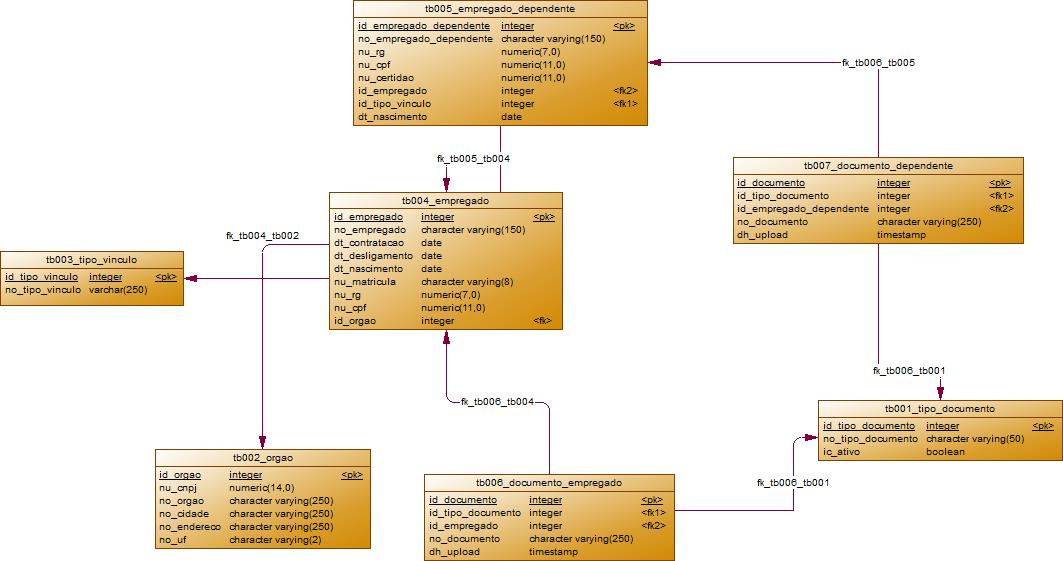
\includegraphics[width=0.8\textwidth]{modelo_relacional}
		\end{center}
		\caption{Modelo Relacional }
		\label{fig:modelorelacional}
	\end{figure}
\end{frame}

\begin{frame}{Relacional x NoSQL}
    \begin{itemize}
    \item Armazenamento de dados de forma não relacional;
    \item Schema free;
    \item Chave-Valor / Orientados a Documentos / Orientados a Colunas / Baseados em Grafos;
    \item Google, Amazon, Facebook...
    \item MongoDB, Cassandra, NEO4j, Redis
    \end{itemize}
\end{frame}

\begin{frame}{Relacional x NoSQL}
	\begin{figure}[!htbp]
		\begin{center}
			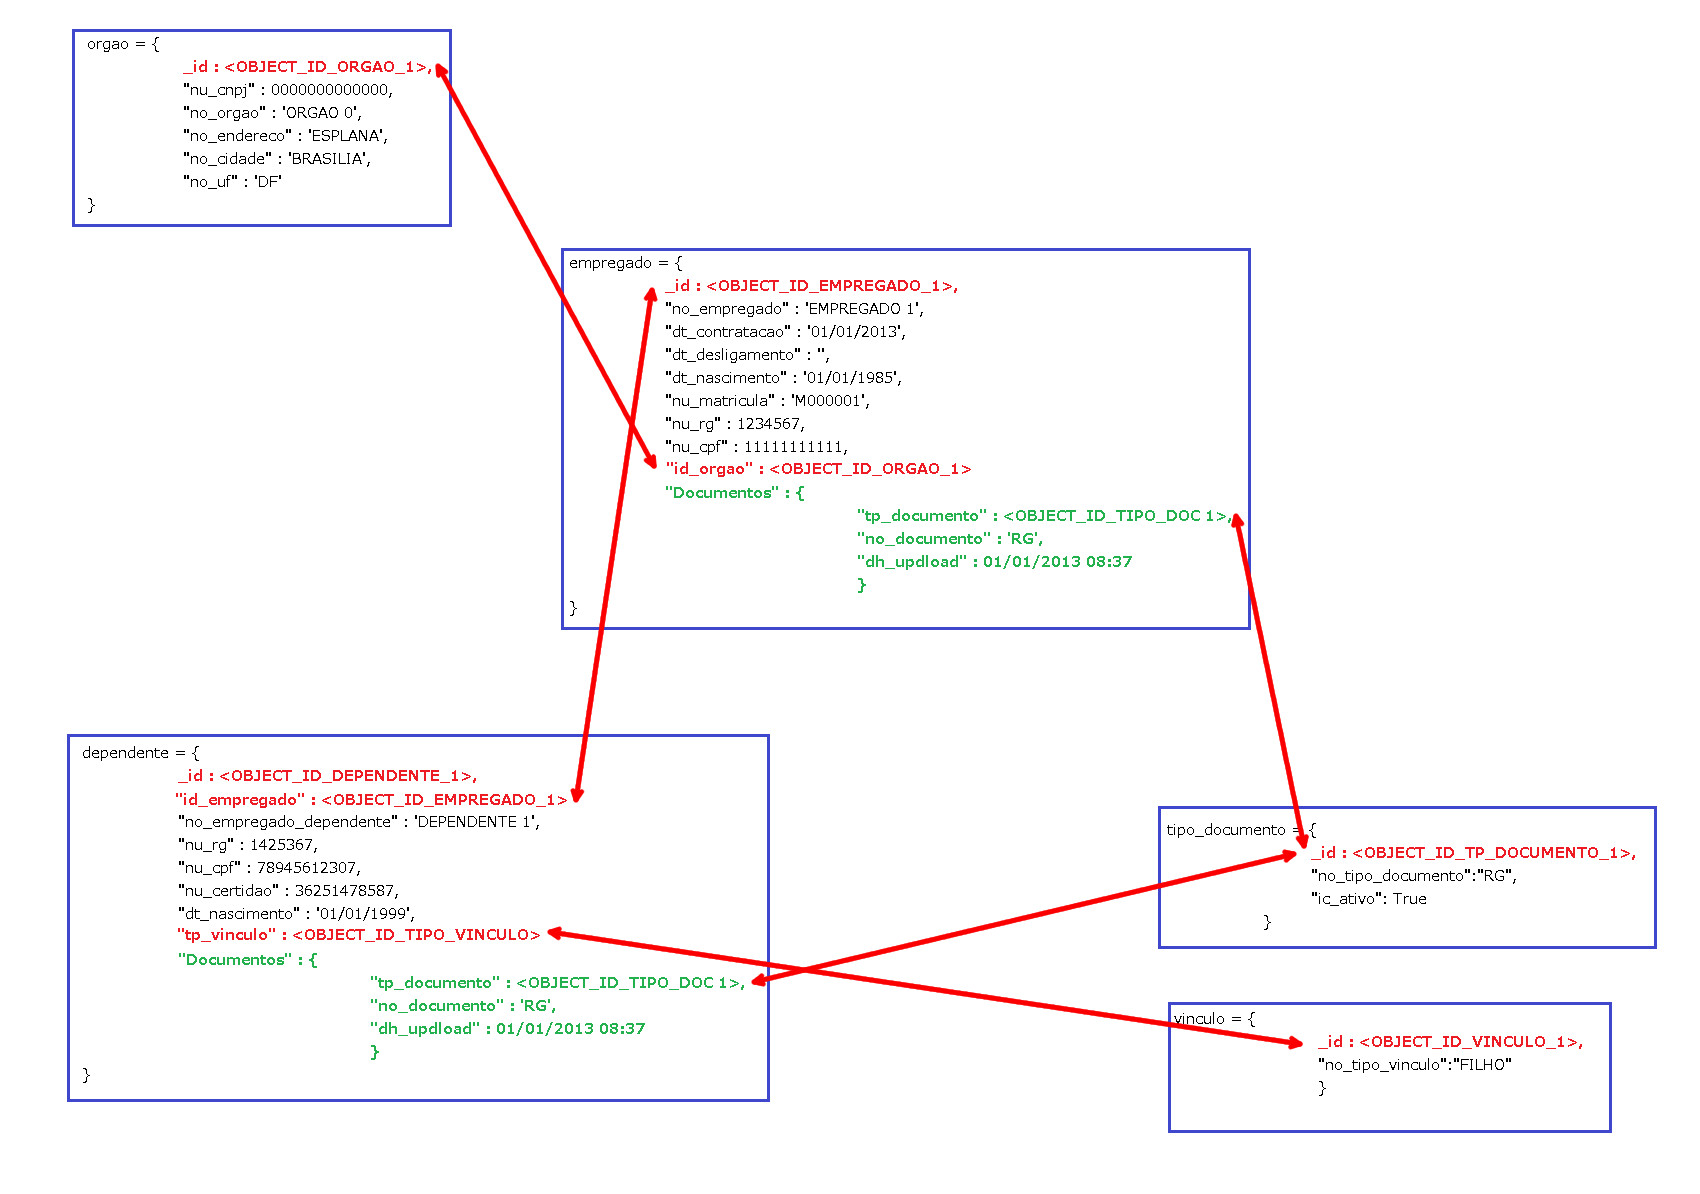
\includegraphics[width=0.6\textwidth]{modelo_orientado_documentos}
		\end{center}
		\caption{ Modelagem orientada a documentos implementada no protótipo.}
		\label{fig:modeloorientadodocumentos}
	\end{figure}
\end{frame}

\section{O Projeto}

\begin{frame}{O Projeto}
    \begin{itemize}
	\item Grande número de pastas funcionais físicas geram custos para manter a qualidade dos arquivos permanentes;
	\item Digitalização das pastas funcionais;
    \end{itemize}
\end{frame}

\begin{frame}{O Projeto}
    \begin{itemize}
	\item AFD - Criação de um dossiê, em mídia digital;
	\item Fonte Primária de informações cadastrais do Servidor Público Civil Federal. \textit{citar site do SIGEPE}
    \end{itemize}
\end{frame}

\begin{frame}{Problema}
    \begin{itemize}
           \item Determinar se um banco de dados NoSQL é indicado para um caso como o citado e se temos um tipo de banco mais adequado.
    \end{itemize}
\end{frame}


%\begin{frame}{Hipótese}
%    \begin{itemize}
%           \item Podemos melhorar a performance nas consultas e armazenamento, porém o grau de consistência e confiabilidade necessários devem ser medidos e implementados na aplicação.
%    \end{itemize}
%\end{frame}


\begin{frame}{Motivação}
    \begin{itemize}
    \item Tema relativamente novo;
    \item Caso Real;
    \item Mercado -> Academia;
    \item Novas Tecnologias;
    \end{itemize}
\end{frame}


\begin{frame}{Objetivo Geral}
    \begin{itemize}
    \item Comparar os modelos relacional e não relacional (Orientada a Documento) de armazenamento  para o contexto do Assentamento Digital Funcional (AFD).
    \end{itemize}
\end{frame}


\begin{frame}{Objetivos Específicos}
    \begin{itemize}
    \item Compreender, abstrair e modelar os conceitos e operações do AFD;
    \item Modelar os conceitos do AFD utilizando a estratégia relacional;
    \item Modelar os conceitos do AFD utilizando a estratégia orientada a documentos;
    \item Implementar os modelos em SGBDs relacionais e orientados a documentos;
%    \item Implementar uma arquitetura SOA para realizar as operações do AFD, utilizando os dois bancos para a persistência;
%   \item Projetar, implementar e realizar testes de desempenho que nos permitam tirar conclusões sobre quais dos modelos são mais %propícios para o armazenamento dos dados do AFD.
    \end{itemize}
\end{frame}

\begin{frame}{Objetivos Específicos}
    \begin{itemize}
    \item Implementar uma arquitetura SOA para realizar as operações do AFD, utilizando os dois bancos para a persistência;
   \item Projetar, implementar e realizar testes de desempenho que nos permitam tirar conclusões sobre quais dos modelos são mais propícios para o armazenamento dos dados do AFD.
    \end{itemize}
\end{frame}

\begin{frame}{Resultados Esperados}
    \begin{itemize}
    \item Obter informações o bastante para escolher o banco de dados mais indicado para esse caso e semelhantes.
    \end{itemize}
\end{frame}


\begin{frame}{Teste de Software}
    \begin{itemize}
    \item Qualidade de software;
    \item Teste: atividades nas quais um sistema ou um componente é executado sob determinadas
condições e os resultados são observados ou gravados, e uma avaliação é
feita observando determinado comportamento do sistema ou do componente; 
    \item Vários tipos: Testes de sistema, usabilidade, back-to-back, carga, performance.
    \item Com a complexidade e tamanho das aplicações os testes manuais se tornaram inviáveis.
    \item Solução: Testes automatizados.
    \end{itemize}
\end{frame}

\begin{frame}{Protótipo AFD}
    \begin{itemize}
    \item Arquitetura SOA;
    \item Principais capacidades para manter os dados do AFD;
    \item Inserção e consulta de órgãos, empregados, dependentes, documentos;
    \item Empregados ativos;
    \item Desligamento de empregados e exclusão de dependentes.
    \end{itemize}
\end{frame}

\begin{frame}{Arquitetura}
	\begin{figure}[!htbp]
		\begin{center}
			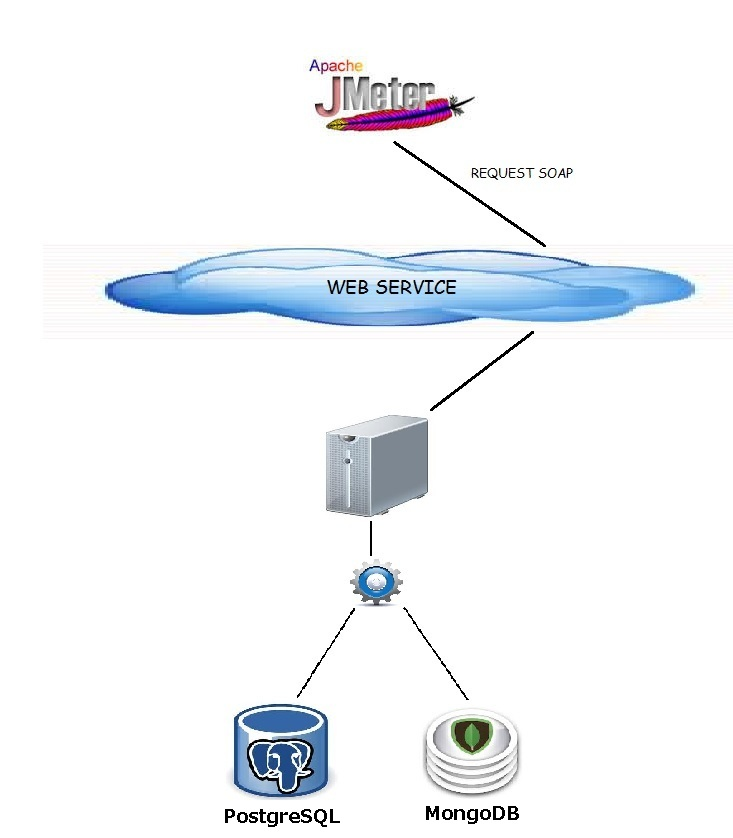
\includegraphics[width=0.4\textwidth]{arquitetura}
		\end{center}
		\caption{Arquitetura de Testes}
		\label{fig:arquitetura}
	\end{figure}
\end{frame}

\begin{frame}{Plano de testes}
    \begin{itemize}
    \item Criação de um plano de testes para as principais capacidades do protótipo;
    \item Plano de testes parametrizáveis : Usuários virtuais, carga de dados via arquivo CSV;
    \item Monitoramento dos resultados;
    \item Geração de gráficos;
    \end{itemize}
\end{frame}

\begin{frame}{Execução dos testes}
    \begin{itemize}
    \item Criação de um plano de testes para as principais capacidades do protótipo;
    \item Plano de testes parametrizáveis : Usuários virtuais, carga de dados via arquivo CSV;
    \item Monitoramento dos resultados;
    \item Geração de gráficos;
    \item As capacidades foram testadas com 10, 100 e, quando possível, com 500 usuários simultâneos;
    \end{itemize}
\end{frame}

\begin{frame}{Execução dos testes}
Os testes foram realizados em uma máquina física com as seguintes configurações:

\begin{itemize}
\item Sistema Operacional: Debian GNU/Linux 6.0
\item Processador: Intel Pentium Quad Core
\item Quantidade de Memória RAM: 4 GB
\item MongoDB: Versão 2.4.0 padrão
\item PostgreSQL: Versão 8.4.16 padrão
\item Driver Python MongoDB: pymongo
\item Driver Python PostgreSQL: psycopg
\end{itemize}
\end{frame}

\begin{frame}{Massa de dados}
\begin{itemize}
\item Quantidade de unidades pagadoras (órgãos): 10
\item Quantidade de empregados por orgão: 100
\item Quantidade de dependentes por empregado: 2 
\item Quantidade de documentos por empregado: 5
\item Quantidade de documentos por dependente: 2
\item Quantidade de dependentes excluídos: 250
\item Quantidade de empregados desligados: 250
\end{itemize}
\end{frame}

\begin{frame}{Métrica}
\begin{itemize}
\item Tempo de Resposta [molineux][raj jain]
\end{itemize}
\end{frame}

\section{Resultados}

\begin{frame}{Resultados}
\begin{figure}[!htbp]
	\begin{center}
		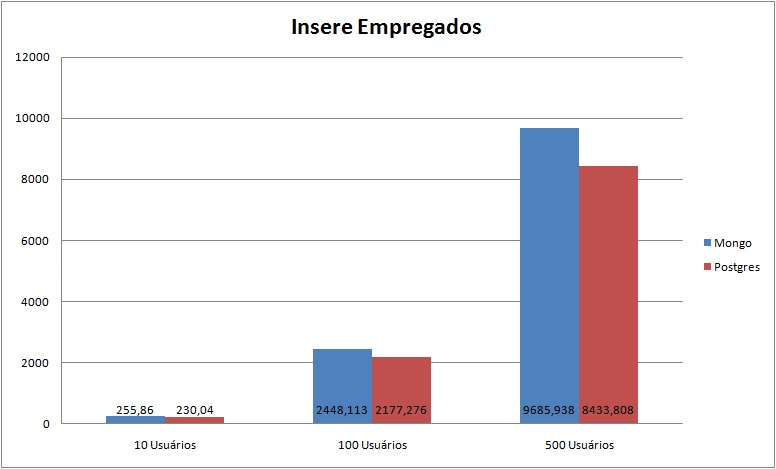
\includegraphics[width=0.8\textwidth]{insere_empregados}
	\end{center}
	\caption{Resultados - Insere Empregados}
	\label{fig:resultinsereempregados}
\end{figure}
\end{frame}

\begin{frame}{Resultados}
\begin{figure}[!htbp]
	\begin{center}
		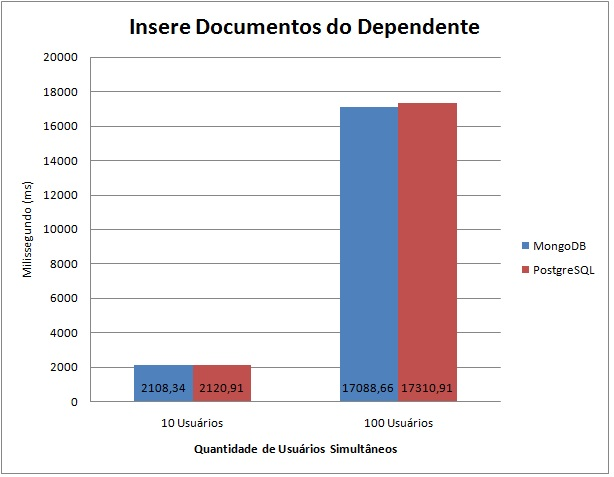
\includegraphics[width=0.6\textwidth]{insere_doc_dependentes}
	\end{center}
	\caption{Resultados - Insere Documento do Dependente}
	\label{fig:resultinseredocdependente}
\end{figure}
\end{frame}

\begin{frame}{Resultados}
\begin{figure}[!htbp]
	\begin{center}
		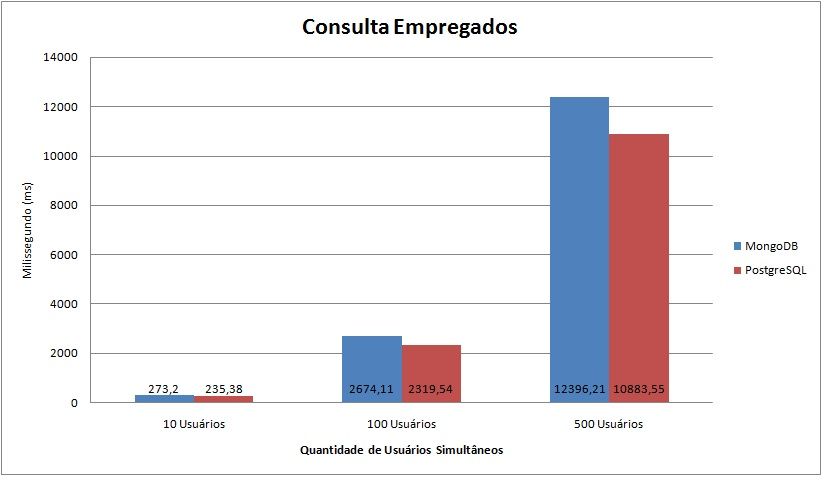
\includegraphics[width=0.8\textwidth]{consulta_empregados}
	\end{center}
	\caption{Resultados - Lista Empregados}
	\label{fig:resultlistaempregados}
\end{figure}
\end{frame}

\begin{frame}{Resultados}
\begin{figure}[!htbp]
	\begin{center}
		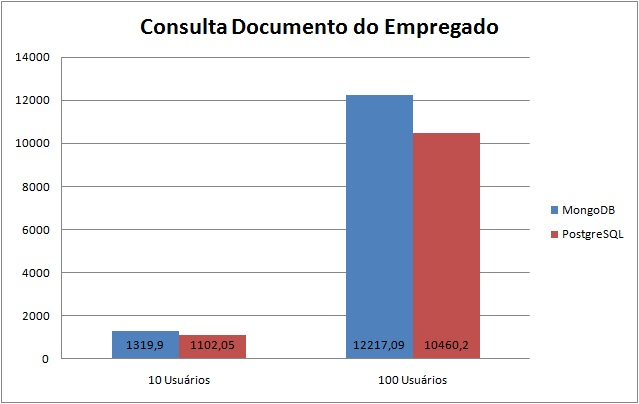
\includegraphics[width=0.6\textwidth]{consulta_doc_empregado}
	\end{center}
	\caption{Resultados - Lista Documentos do Empregado}
	\label{fig:resultlistadocempregado}
\end{figure}
\end{frame}

\begin{frame}{Resultados}
\begin{figure}[!htbp]
	\begin{center}
		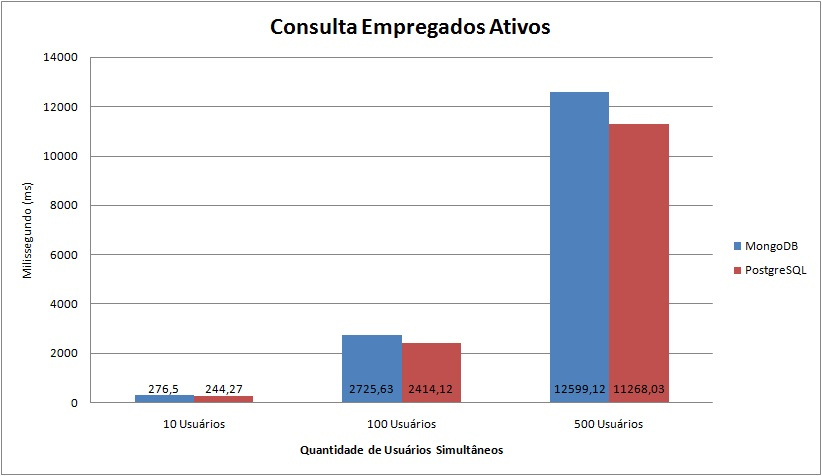
\includegraphics[width=0.8\textwidth]{consulta_estatistica}
	\end{center}
	\caption{Resultados - Consulta Empregados Ativos}
	\label{fig:resultlistaempregadosativos}
\end{figure}
\end{frame}

\begin{frame}{Resultados}
\begin{figure}[!htbp]
	\begin{center}
		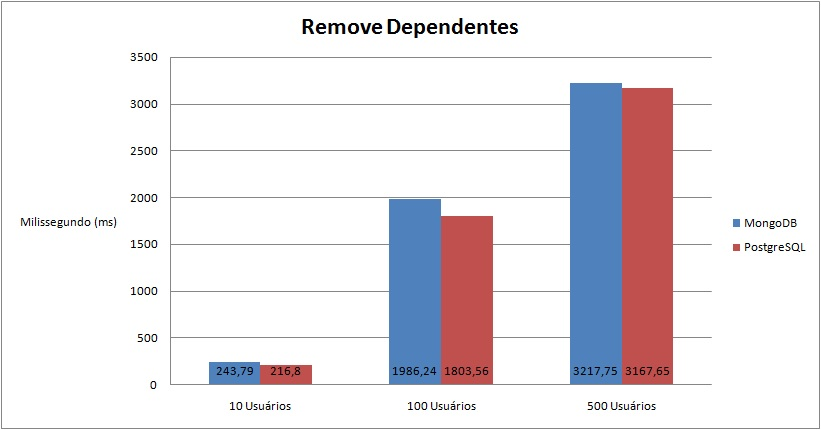
\includegraphics[width=0.8\textwidth]{remove_dependentes}
	\end{center}
	\caption{Resultados - Remove Dependentes}
	\label{fig:resultremovedependentes}
\end{figure}
\end{frame}

\begin{frame}{Resultados}
\begin{figure}[!htbp]
	\begin{center}
		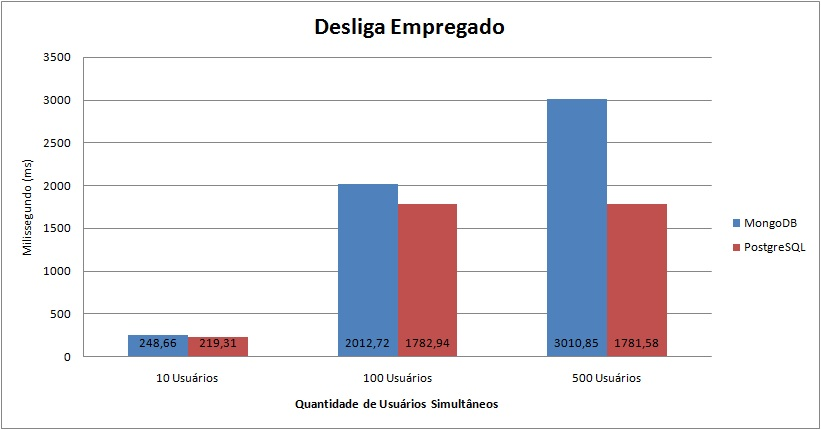
\includegraphics[width=0.8\textwidth]{desliga_empregado}
	\end{center}
	\caption{Resultados - Desliga Empregado}
	\label{fig:resultdesliga_empregado}
\end{figure}
\end{frame}

\begin{frame}{Resultados}
Ao final dos testes pode-se verificar que nenhum banco de dados foi consideravelmente mais veloz que o outro e que, para praticamente todos os testes realizados, o PostgreSQL se mostrou mais rápido. Dessa maneira, para o cenário de manutenção dos dados do AFD, com a arquitetura, massa de dados e modelagem utilizadas, não é vantajoso utilizar o MongoDB para a persistência dos dados, visto que, mesmo com todos os recursos de segurança e controle de transações oferecidos pelo PostgreSQL, ele ainda continua sendo mais performático.
\end{frame}

\section{Considerações Finais e Trabalhos Futuros}

\begin{frame}{Considerações Finais}
\begin{itemize}
\item Cenários definido;
\item Tanto o PostgreSQL quanto o MongoDB possuem seu lugar no mercado;
item Fontes no GitHub;
\end{itemize}
\end{frame}



\begin{frame}{Trabalhos Futuros}
\begin{itemize}
\item Outra modelagem orientada a documentos com uma maior utilização de subdocumentos;
\item Uso de uma arquitetura mais robusta
item Expandir os testes para outros bancos de dados como o MySQL, Cassandra, HBase...
\end{itemize}
\end{frame}




\section{Cronograma}

\newenvironment{changemargin}[2]{%
  \begin{list}{}{%
    \setlength{\topsep}{0pt}%
    \setlength{\leftmargin}{#1}%
    \setlength{\rightmargin}{#2}%
    \setlength{\listparindent}{\parindent}%
    \setlength{\itemindent}{\parindent}%
    \setlength{\parsep}{\parskip}%
  }%
  \item[]}{\end{list}}


\begin{frame}
\begin{changemargin}{-1cm}{-1cm} 
\begin{table}[h]
	\begin{center}
	\begin{tabular}{ p{4cm}lcccccc}
		\hline
			\textbf{Tarefas} & \textbf{JUL} & \textbf{AGO} & \textbf{SET} & \textbf{OUT} & \textbf{NOV} & \textbf{DEZ}\\
		\hline
			Escrita da Monografia & x & x & x & x & x & x\\
			Compreender AFD & x & x &  &  &  & \\
			Modelagem Relacional &  &  & x &  &  & \\
			Modelagem Orientada a  Documentos &  &  & x & x &  & \\
			Implem. Mod. de Dados &  &  & x & x &  & \\
			Arquitetura SOA &  & x & x & x & x & \\
			Projeto e Implem. Testes &  &  & x & x & x & \\
			Execução dos Testes &  &  &  &  & x & x\\
		\hline
	\end {tabular}
	\end{center}
\end{table}
\end{changemargin}
\end{frame}

\section{Referências}

\begin{frame}{Bibliografia I}
\begin{itemize}

\item E. Hewitt. Cassandra: The Definitive Guide. Definitive Guide Series. O'Reilly Media,
2010.

\item S. Tiwari. Professional NoSQL. Wrox Programmer to Programmer. Wiley, 2011.

\item Mongodb oficial site. \url{http://www.mongodb.org/}

\end{itemize}
\end{frame}

\begin{frame}{Bibliografia II}
\begin{itemize}

\item R. Hecht and S. Jablonski. Nosql evaluation: A use case oriented survey. In Cloud
and Service Computing (CSC), 2011 International Conference on, pages 336 - 341,
dec. 2011.
\end{itemize}
\end{frame}

\begin{frame}{Bibliografia III}
\begin{itemize}

\item Vinayak R. Borkar, Michael J. Carey, and Chen Li. Big data platforms: What's
next? XRDS, September 2012.

\item Ricardo W. Brito. Banco de dados nosql x sgbds relacionais: Análise comparativa.
2010.
\end{itemize}
\end{frame}

\begin{frame}\frametitle{Bibliografia}
  % estilo da bibliografia
  \bibliographystyle{abbrv}
  % chamando o arquivo refs.bib
  \bibliography{refs}
\end{frame}

\appendix

\begin{frame}
  \frametitle{Obrigado pela atenção!}
  \begin{center}
    {\Huge Obrigado!}
  \end{center}
\end{frame}
